\documentclass[11pt,a4paper]{article}
\usepackage[utf8]{vietnam}
\usepackage{amsmath,amssymb,mathrsfs}
\usepackage{graphicx}
\usepackage{tikz}
\usepackage{array}
\usepackage[top=1.0cm,bottom=1.8cm,left=1.4cm,right=1.4cm,footskip=0.8cm,headheight=16pt]{geometry}
\usepackage{fancyhdr}
\usepackage{tcolorbox}
\tcbuselibrary{skins}
\usepackage{lastpage}
\usepackage[loigiai]{ex_test}
\graphicspath{{../../Hinh_Anh/NTT_10/}}

\makeatletter
\@ifundefined{c@bt}{\newcounter{bt}}{}
\makeatother

\pagestyle{fancy}
\fancyhf{}
\renewcommand{\headrulewidth}{0pt}
\renewcommand{\footrulewidth}{0.4pt}
\lfoot{\footnotesize\textsl{Lớp Toán Cô Thúy -- SĐT: 0935.322.328 -- 50/2C Phạm Thị Liên}}
\rfoot{\footnotesize\textsl{Trang \thepage/\pageref{LastPage} -- Hướng dẫn giải Mã đề 102}}
\setlength{\parskip}{1pt}
\setlength{\parindent}{0pt}

\begin{document}

\noindent
\begin{tabular}{|p{6.6cm}|p{6.6cm}|>{\centering\arraybackslash}p{3.2cm}|}
\hline
\begin{minipage}{6.6cm}
\vspace{3pt}
\centering
{\large\bfseries\color{blue!80!black} LỚP TOÁN CÔ THÚY}\\[3pt]
\textbf{SĐT:} 0935.322.328\\[2pt]
\textbf{Địa chỉ:} 50/2C Phạm Thị Liên
\vspace{3pt}
\end{minipage}
&
\multicolumn{2}{p{10.2cm}|}{
\begin{minipage}{10.2cm}
\vspace{3pt}
\centering
{\bfseries\color{red!80!black} HƯỚNG DẪN GIẢI CHI TIẾT GIỮA KỲ I}\\[3pt]
\textbf{Môn: VẬT LÍ 10 -- THPT NGUYỄN TRƯỜNG TỘ}\\[2pt]
\textit{Năm học 2025 -- 2026 -- Mã đề: 102}
\vspace{3pt}
\end{minipage}
} \\
\hline
\rule{0pt}{14pt}\textbf{Giáo viên:} HỒ THỊ THÚY &
\rule{0pt}{14pt}\textbf{Môn học:} VẬT LÍ 10 &
\rule{0pt}{14pt}\textbf{Mã đề thi 102}\rule[-4pt]{0pt}{4pt} \\
\hline
\end{tabular}
\vspace{0.1cm}

\vspace{0.15cm}
\begin{flushleft}
	{\color{blue!50!green}\fbox{\fontfamily{qag}\bfseries\selectfont PHẦN I. Câu trắc nghiệm nhiều phương án lựa chọn (3,0 điểm)}}
	\textit{\small (Thí sinh trả lời từ câu 1 đến câu 12. Mỗi câu hỏi thí sinh chỉ chọn một phương án.)}
\end{flushleft}
\setcounter{ex}{0}
\setcounter{bt}{0}

% Câu 1
\begin{ex}
	Công thức tính vận tốc của chuyển động thẳng biến đổi đều là $v = v_0 + at$. Đối với chuyển động thẳng nhanh dần đều thì ta luôn có
	\choice
	{$v$ luôn dương}
	{$a$ luôn dương}
	{\True $a$ luôn cùng dấu với $v$}
	{$a$ luôn ngược dấu với $v$}
	\loigiai{
		Trong chuyển động thẳng nhanh dần đều, vectơ gia tốc $\vec{a}$ luôn cùng hướng với vectơ vận tốc $\vec{v}$, do đó $a$ và $v$ luôn cùng dấu ($a \cdot v > 0$).\par
	}
\end{ex}

% Câu 2
\begin{ex}
	Đặc điểm nào sau đây \textbf{không} phải là tính chất của vectơ vận tốc trong chuyển động thẳng của một chất điểm?
	\choice
	{Gốc nằm trên chất điểm chuyển động}
	{Phương trùng với phương chuyển động của chất điểm}
	{\True Có chiều luôn ngược với chiều chuyển động của chất điểm}
	{Độ dài tỉ lệ với độ lớn của vận tốc theo một tỉ xích quy ước}
	\loigiai{
		Vectơ vận tốc $\vec{v}$ luôn có hướng (gồm phương và chiều) trùng với hướng chuyển động của chất điểm. Phát biểu C nói chiều ngược với chiều chuyển động là sai.\par
	}
\end{ex}

% Câu 3
\begin{ex}
	Chọn phát biểu đúng khi nói về quãng đường đi được của một vật chuyển động.
	\choice
	{\True Quãng đường là một đại lượng vô hướng luôn nhận giá trị không âm ($s \ge 0$)}
	{Quãng đường luôn luôn nhận giá trị âm}
	{Quãng đường là một đại lượng vectơ xác định hướng chuyển động}
	{Quãng đường có thể nhận giá trị âm hoặc dương tùy thuộc vào chiều dương được chọn}
	\loigiai{
		Quãng đường đi được $s$ là độ dài cung đường mà vật vạch ra trong quá trình chuyển động, là đại lượng vô hướng và luôn không âm ($s \ge 0$).\par
	}
\end{ex}

% Câu 4
\begin{ex}
	Gọi $\overline{A}$ là giá trị trung bình, $\Delta A'$ là sai số dụng cụ, $\overline{\Delta A}$ là sai số ngẫu nhiên tuyệt đối. Công thức tính sai số tuyệt đối toàn phần $\Delta A$ của phép đo trực tiếp là
	\choice
	{\True $\Delta A = \overline{\Delta A} + \Delta A'$}
	{$\Delta A = \overline{\Delta A} - \Delta A'$}
	{$\Delta A = \overline{\Delta A} \cdot \Delta A'$}
	{$\Delta A = \overline{\Delta A} / \Delta A'$}
	\loigiai{
		Sai số tuyệt đối toàn phần của một phép đo trực tiếp bằng tổng của sai số ngẫu nhiên và sai số dụng cụ: $\Delta A = \overline{\Delta A} + \Delta A'$.\par
	}
\end{ex}

% Câu 5
\begin{ex}
	Một vật chuyển động trên đường thẳng có vận tốc $v$ và gia tốc $a$. Chuyển động của vật là chuyển động chậm dần đều khi
	\choice
	{gia tốc $a < 0$}
	{gia tốc $a > 0$}
	{\True tích số $a \cdot v < 0$}
	{vận tốc $v < 0$}
	\loigiai{
		Chuyển động thẳng là chậm dần đều khi vectơ gia tốc ngược hướng với vectơ vận tốc, tương ứng tích số giữa hai giá trị đại số mang dấu âm: $a \cdot v < 0$.\par
	}
\end{ex}

% Câu 6
\begin{ex}
	Những phân ngành nào sau đây thuộc về các lĩnh vực nghiên cứu nền tảng của khoa học Vật lí cổ điển?
	\choice
	{Cơ học, nhiệt học, cấu trúc tiến hóa của vật chất vô cơ}
	{Nhiệt học, quang học, cơ chế di truyền của sinh vật học}
	{\True Cơ học, nhiệt học, điện học, quang học}
	{Điện học, quang học, tính chất hóa học của hợp chất}
	\loigiai{
		Cơ học, nhiệt học, điện học và quang học là bốn phân ngành nền tảng cốt lõi của Vật lí học cổ điển.\par
	}
\end{ex}

% Câu 7
\begin{ex}
	Biển báo dùng để cảnh báo nguy cơ gây ô nhiễm nguy hiểm đối với môi trường sinh thái là biển báo nào trong hình dưới đây?
	\begin{center}
		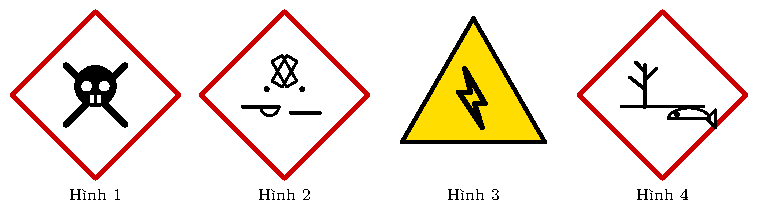
\includegraphics[width=12.0cm]{fig_cau7_bienbao.pdf}
	\end{center}
	\choice
	{Hình 1 (Chất độc cấp tính)}
	{Hình 2 (Chất ăn mòn)}
	{Hình 3 (Nguy cơ điện giật)}
	{\True Hình 4 (Nguy hại môi trường)}
	\loigiai{
		Biển báo Hình 4 (biểu tượng cây khô trơ trụi và cá chết) là kí hiệu tiêu chuẩn cảnh báo chất độc nguy hại đối với môi trường sinh thái.\par
	}
\end{ex}

% Câu 8
\begin{ex}
	Một người chạy bộ dọc theo một đường thẳng, trong khoảng thời gian $10\text{ s}$ người đó chạy được quãng đường $150\text{ m}$. Tốc độ trung bình của người đó là
	\choice
	{$150\text{ m/s}$}
	{$0{,}015\text{ m/s}$}
	{\True $15\text{ m/s}$}
	{$15\text{ km/s}$}
	\loigiai{
		Tốc độ trung bình:\par
		\[v_{\text{tb}} = \frac{s}{t} = \frac{150}{10} = 15\text{ m/s}.\]
	}
\end{ex}

% Câu 9
\begin{ex}
	Một ô tô đang chuyển động thẳng đều thì hãm phanh để dừng lại. Chọn chiều dương là chiều chuyển động của xe. Nhận xét nào sau đây đúng về dấu của vận tốc $v$ và gia tốc $a$?
	\choice
	{$a > 0,\ v > 0$}
	{$a < 0,\ v < 0$}
	{$a > 0,\ v < 0$}
	{\True $a < 0,\ v > 0$}
	\loigiai{
		-- Xe chuyển động theo chiều dương nên $v > 0$.\par
		-- Xe hãm phanh chuyển động chậm dần đều nên gia tốc ngược chiều vận tốc, suy ra $a < 0$.\par
	}
\end{ex}

% Câu 10
\begin{ex}
	Chọn mốc thời gian là lúc $t_0 = 8\text{ h}$. Một chuyển động kéo dài trong khoảng thời gian $\Delta t = 3\text{ h}$. Thời điểm kết thúc chuyển động là lúc
	\choice
	{$8\text{ h}$}
	{$10\text{ h}$}
	{\True $11\text{ h}$}
	{$12\text{ h}$}
	\loigiai{
		Thời điểm kết thúc: $t = t_0 + \Delta t = 8\text{ h} + 3\text{ h} = 11\text{ h}$.\par
	}
\end{ex}

% Câu 11
\begin{ex}
	Đồ thị độ dịch chuyển -- thời gian $(d - t)$ của một xe chuyển động thẳng có dạng đường thẳng dốc xuống từ vạch $80\text{ km}$ về vạch $0\text{ km}$ trong thời gian $2\text{ h}$ như đường (2) ở hình bên. Kết luận nào sau đây đúng?
	\begin{center}
		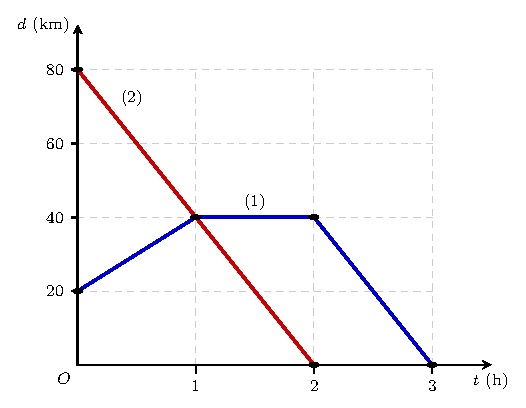
\includegraphics[width=6.5cm]{fig_dothi_xe12.pdf}
	\end{center}
	\choice
	{\True Vật chuyển động thẳng đều ngược chiều dương với tốc độ $40\text{ km/h}$}
	{Vật chuyển động thẳng đều cùng chiều dương với tốc độ $20\text{ km/h}$}
	{Vật chuyển động thẳng đều ngược chiều dương với tốc độ $60\text{ km/h}$}
	{Vật chuyển động thẳng đều cùng chiều dương với tốc độ $40\text{ km/h}$}
	\loigiai{
		-- Đồ thị dốc xuống cho thấy độ dịch chuyển giảm theo thời gian, vật chuyển động ngược chiều dương.\par
		-- Tốc độ của vật: $v = \dfrac{|\Delta d|}{\Delta t} = \dfrac{|0 - 80|}{2} = 40\text{ km/h}$.\par
	}
\end{ex}

% Câu 12
\begin{ex}
	Khi được thả rơi cùng một lúc từ cùng một độ cao trong không khí, chuyển động của vật nào sau đây được coi gần đúng là rơi tự do?
	\choice
	{Một chiếc khăn voan mỏng nhẹ}
	{Một sợi chỉ mảnh dài}
	{Một chiếc lá cây khô đang rụng}
	{\True Một viên sỏi nhỏ đặc}
	\loigiai{
		Viên sỏi nhỏ đặc có khối lượng riêng lớn, lực cản của không khí tác dụng lên nó là không đáng kể so với trọng lượng, nên chuyển động của nó được coi gần đúng là sự rơi tự do.\par
	}
\end{ex}

\vspace{0.15cm}
\begin{flushleft}
	{\color{blue!50!green}\fbox{\fontfamily{qag}\bfseries\selectfont PHẦN II. Câu trắc nghiệm đúng sai (2,0 điểm)}}
	\textit{\small (Thí sinh trả lời từ câu 1 đến câu 2. Trong mỗi ý a), b), c), d) ở mỗi câu, thí sinh chọn đúng hoặc sai.)}
\end{flushleft}
\setcounter{ex}{0}
\setcounter{bt}{0}

% Phần II Câu 1
\begin{ex}
	Hình bên mô tả đồ thị độ dịch chuyển -- thời gian $(d - t)$ của hai xe 1 và xe 2 cùng chuyển động thẳng dọc theo trục tọa độ $Ox$.
	\begin{center}
		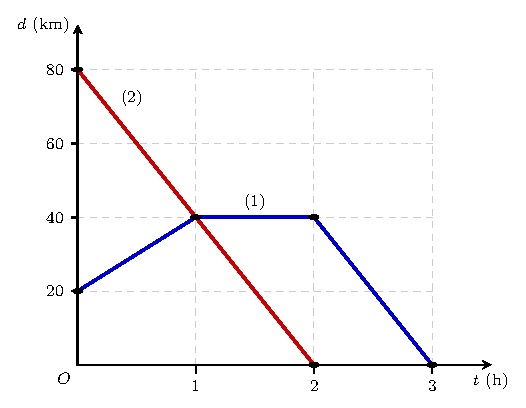
\includegraphics[width=6.5cm]{fig_dothi_xe12.pdf}
	\end{center}
	\choiceTF[t]
	{\True Trong khoảng thời gian từ $1\text{ h}$ đến $2\text{ h}$, xe 1 đứng yên không chuyển động.}
	{Xe 2 luôn duy trì chuyển động thẳng đều theo chiều dương trong suốt khoảng thời gian từ $0\text{ h}$ đến $2\text{ h}$.}
	{Trong khoảng thời gian từ $1\text{ h}$ đến $2\text{ h}$, xe 1 và xe 2 chuyển động với cùng vận tốc.}
	{\True Trong khoảng thời gian từ $0\text{ h}$ đến $1\text{ h}$, xe 1 chuyển động thẳng đều theo chiều dương với tốc độ $20\text{ km/h}$.}
	\loigiai{
		{\color{green!50!black}\textbf{a) Đúng.}} Từ $1\text{ h}$ đến $2\text{ h}$, đường (1) nằm ngang song song trục thời gian ở $d = 40\text{ km}$, chứng tỏ xe 1 đứng yên.\par
		{\color{red!80!black}\textbf{b) Sai.}} Đường (2) dốc xuống từ $80\text{ km}$ về $0\text{ km}$, chứng tỏ xe 2 chuyển động ngược chiều dương.\par
		{\color{red!80!black}\textbf{c) Sai.}} Từ $1\text{ h}$ đến $2\text{ h}$, xe 1 đứng yên ($v_1 = 0$) còn xe 2 vẫn chuyển động ngược chiều dương ($v_2 = -40\text{ km/h}$), do đó vận tốc khác nhau.\par
		{\color{green!50!black}\textbf{d) Đúng.}} Từ $0\text{ h}$ đến $1\text{ h}$, xe 1 đi từ $d = 20\text{ km}$ đến $d = 40\text{ km}$. Vận tốc $v = \dfrac{40 - 20}{1} = 20\text{ km/h} > 0$.\par
	}
\end{ex}

% Phần II Câu 2
\begin{ex}
	Một vật nặng được thả rơi tự do từ trạng thái nghỉ tại độ cao $45\text{ m}$ so với mặt đất. Bỏ qua lực cản của không khí và lấy gia tốc trọng trường $g = 10\text{ m/s}^2$.
	\choiceTF[t]
	{\True Phương chuyển động rơi của vật luôn hướng theo phương thẳng đứng.}
	{Thời gian rơi toàn phần để vật chạm đất bằng $2{,}5\text{ s}$.}
	{\True Quãng đường vật rơi được sau $2\text{ s}$ đầu tiên kể từ lúc thả bằng $20\text{ m}$.}
	{\True Thời gian vật rơi trong $13{,}75\text{ m}$ cuối cùng ngay trước khi chạm đất bằng $0{,}5\text{ s}$.}
	\loigiai{
		{\color{green!50!black}\textbf{a) Đúng.}} Chuyển động rơi tự do có phương thẳng đứng, chiều từ trên xuống dưới.\par
		{\color{red!80!black}\textbf{b) Sai.}} Thời gian rơi chạm đất: $t = \sqrt{\dfrac{2h}{g}} = \sqrt{\dfrac{2 \cdot 45}{10}} = 3\text{ s} \ne 2{,}5\text{ s}$.\par
		{\color{green!50!black}\textbf{c) Đúng.}} Quãng đường sau $2\text{ s}$ đầu: $s = \dfrac{1}{2}gt^2 = \dfrac{1}{2} \cdot 10 \cdot 2^2 = 20\text{ m}$.\par
		{\color{green!50!black}\textbf{d) Đúng.}} Vật rơi $45 - 13{,}75 = 31{,}25\text{ m}$ đầu tiên mất thời gian $t_1 = \sqrt{\dfrac{2 \cdot 31{,}25}{10}} = 2{,}5\text{ s}$. Do đó thời gian rơi đoạn cuối là $\Delta t = 3 - 2{,}5 = 0{,}5\text{ s}$.\par
	}
\end{ex}

\vspace{0.15cm}
\begin{flushleft}
	{\color{blue!50!green}\fbox{\fontfamily{qag}\bfseries\selectfont PHẦN III. Câu trắc nghiệm trả lời ngắn (2,0 điểm)}}
	\textit{\small (Thí sinh trả lời từ câu 1 đến câu 4.)}
\end{flushleft}
\setcounter{ex}{0}
\setcounter{bt}{0}

% Phần III Câu 1
\begin{ex}
	Một ô tô chuyển động thẳng nhanh dần đều. Sau thời gian $\Delta t = 8\text{ s}$, vận tốc của ô tô tăng đều từ $5\text{ m/s}$ đến $9\text{ m/s}$. Tính quãng đường mà ô tô đi được trong khoảng thời gian trên theo đơn vị kilômét (km)?
	\par\shortans[oly]{0,056}
	\loigiai{
		Gia tốc của ô tô: $a = \dfrac{v - v_0}{\Delta t} = \dfrac{9 - 5}{8} = 0{,}5\text{ m/s}^2$.\par
		Quãng đường ô tô đi được theo đơn vị mét:\par
		\[s = v_0 t + \frac{1}{2}at^2 = 5 \cdot 8 + \frac{1}{2} \cdot 0{,}5 \cdot 8^2 = 40 + 16 = 56\text{ m}.\]
		Đổi sang kilômét: $s = \dfrac{56}{1000} = 0{,}056\text{ km}$.\par
	}
\end{ex}

% Phần III Câu 2
\begin{ex}
	Một ô tô di chuyển chặng thứ nhất đi được quãng đường $24\text{ km}$ về hướng Đông, sau đó rẽ sang hướng Bắc chạy tiếp một đoạn $7\text{ km}$ thì dừng lại. Độ lớn độ dịch chuyển tổng hợp của ô tô sau cả hai chặng là bao nhiêu kilômét (km)?
	\par\shortans[oly]{25}
	\loigiai{
		Hai hướng chuyển động Đông và Bắc vuông góc với nhau.\par
		Độ lớn độ dịch chuyển tổng hợp:\par
		\[d = \sqrt{d_1^2 + d_2^2} = \sqrt{24^2 + 7^2} = \sqrt{576 + 49} = \sqrt{625} = 25\text{ km}.\]
	}
\end{ex}

% Phần III Câu 3
\begin{ex}
	Một vật được thả rơi tự do từ một độ cao $h$ xuống mặt đất. Lấy $g = 10\text{ m/s}^2$. Trong $1\text{ s}$ cuối cùng ngay trước khi chạm đất, vật rơi được quãng đường $25\text{ m}$. Thời gian rơi toàn phần của vật cho đến khi chạm đất là bao nhiêu giây?
	\par\shortans[oly]{3}
	\loigiai{
		Gọi $t$ là tổng thời gian rơi chạm đất của vật ($t > 1\text{ s}$).\par
		Quãng đường vật rơi trong $1\text{ s}$ cuối cùng:\par
		\[\Delta s = s(t) - s(t - 1) = \frac{1}{2}gt^2 - \frac{1}{2}g(t - 1)^2 = g\left(t - 0{,}5\right).\]
		Thay số: $25 = 10(t - 0{,}5) \Rightarrow t - 0{,}5 = 2{,}5 \Rightarrow t = 3\text{ s}$.\par
	}
\end{ex}

% Phần III Câu 4
\begin{ex}
	Một người đi xe máy đang chuyển động thẳng đều với vận tốc $12\text{ m/s}$ thì hãm phanh. Xe chuyển động thẳng chậm dần đều rồi dừng lại sau khi đi thêm được đoạn đường $7{,}2\text{ m}$. Chọn chiều dương là chiều chuyển động, gia tốc của xe máy bằng bao nhiêu $\text{m/s}^2$?
	\par\shortans[oly]{-10}
	\loigiai{
		Vận tốc đầu $v_0 = 12\text{ m/s}$, vận tốc cuối khi dừng hẳn $v = 0$.\par
		Áp dụng hệ thức liên hệ độc lập thời gian:\par
		\[v^2 - v_0^2 = 2as \Rightarrow 0^2 - 12^2 = 2 \cdot a \cdot 7{,}2 \Rightarrow -144 = 14{,}4a \Rightarrow a = -10\text{ m/s}^2.\]
	}
\end{ex}

\vspace{0.15cm}
\begin{flushleft}
	{\color{blue!50!green}\fbox{\fontfamily{qag}\bfseries\selectfont PHẦN IV. Tự luận (3,0 điểm)}}
	\textit{\small (Thí sinh trình bày lời giải từ câu 1 đến câu 3.)}
\end{flushleft}
\setcounter{ex}{0}
\setcounter{bt}{0}

% Phần IV Câu 1
\begin{ex}
	Một chiếc thuyền máy chuyển động trên một dòng sông từ bến $A$ đến bến $B$ cách nhau $6\text{ km}$, sau đó quay đầu chạy ngược dòng từ $B$ về lại bến $A$. Tổng thời gian cả đi lẫn về là $2\text{ giờ } 30\text{ phút}$. Biết vận tốc của dòng nước đối với bờ sông ổn định và bằng $5\text{ km/h}$.
	\par \textbf{a)} Tính vận tốc của thuyền máy đối với dòng nước (theo đơn vị $\text{km/h}$, làm tròn đến hai chữ số thập phân). \par \textbf{b)} Hỏi khi thuyền đi xuôi dòng nước mất khoảng thời gian bao nhiêu giờ (làm tròn đến hai chữ số thập phân)?
	\loigiai{
		Đổi: $2\text{ giờ } 30\text{ phút} = 2{,}5\text{ h}$.\par
		\textbf{a)} Gọi $v$ là vận tốc của thuyền máy đối với dòng nước ($v > 5\text{ km/h}$).\par
		-- Vận tốc khi xuôi dòng: $v_1 = v + 5\text{ (km/h)}$; thời gian xuôi dòng: $t_1 = \dfrac{6}{v + 5}\text{ (h)}$.\par
		-- Vận tốc khi ngược dòng: $v_2 = v - 5\text{ (km/h)}$; thời gian ngược dòng: $t_2 = \dfrac{6}{v - 5}\text{ (h)}$.\par
		Phương trình tổng thời gian chuyển động:\par
		\[t_1 + t_2 = 2{,}5 \Rightarrow \frac{6}{v + 5} + \frac{6}{v - 5} = 2{,}5 \Rightarrow \frac{12v}{v^2 - 25} = 2{,}5.\]
		\[\Rightarrow 2{,}5v^2 - 12v - 62{,}5 = 0 \Leftrightarrow 5v^2 - 24v - 125 = 0.\]
		Giải phương trình bậc hai với điều kiện $v > 5$, ta nhận nghiệm dương:\par
		\[v = \frac{12 + \sqrt{12^2 - 5 \cdot (-125)}}{5} = \frac{12 + \sqrt{769}}{5} \approx 7{,}95\text{ km/h}.\]
		\textbf{b)} Thời gian thuyền máy đi xuôi dòng nước:\par
		\[t_1 = \frac{6}{v + 5} \approx \frac{6}{7{,}95 + 5} = \frac{6}{12{,}95} \approx 0{,}46\text{ h} \text{ (khoảng } 27{,}8\text{ phút)}.\]
	}
\end{ex}

% Phần IV Câu 2
\begin{ex}
	Bảng số liệu dưới đây ghi lại thời gian rơi tự do của một vật giữa hai điểm cố định trong phòng thí nghiệm qua 5 lần đo:
	\par \textbf{a)} Tính giá trị trung bình $\overline{t}$ của thời gian rơi. \par \textbf{b)} Xác định sai số tuyệt đối trung bình $\overline{\Delta t}$ của phép đo.
	\loigiai{
		\begin{center}\begin{tabular}{|c|c|c|c|c|c|}\hline \textbf{Lần đo} & \textbf{Lần 1} & \textbf{Lần 2} & \textbf{Lần 3} & \textbf{Lần 4} & \textbf{Lần 5} \\ \hline \textbf{Thời gian rơi (s)} & 0{,}315 & 0{,}318 & 0{,}316 & 0{,}317 & 0{,}319 \\ \hline\end{tabular}\end{center}\par
		\textbf{a)} Giá trị trung bình của thời gian rơi qua 5 lần đo:\par
		\[\overline{t} = \frac{0{,}315 + 0{,}318 + 0{,}316 + 0{,}317 + 0{,}319}{5} = \frac{1{,}585}{5} = 0{,}317\text{ s}.\]
		\textbf{b)} Sai số tuyệt đối của từng lần đo:\par
		\[\Delta t_1 = |0{,}317 - 0{,}315| = 0{,}002\text{ s}; \quad \Delta t_2 = |0{,}317 - 0{,}318| = 0{,}001\text{ s};\]
		\[\Delta t_3 = |0{,}317 - 0{,}316| = 0{,}001\text{ s}; \quad \Delta t_4 = |0{,}317 - 0{,}317| = 0{,}000\text{ s}; \quad \Delta t_5 = |0{,}317 - 0{,}319| = 0{,}002\text{ s}.\]
		Sai số tuyệt đối trung bình của phép đo:\par
		\[\overline{\Delta t} = \frac{0{,}002 + 0{,}001 + 0{,}001 + 0{,}000 + 0{,}002}{5} = \frac{0{,}006}{5} = 0{,}0012\text{ s}.\]
	}
\end{ex}

% Phần IV Câu 3
\begin{ex}
	Một vật bắt đầu chuyển động thẳng nhanh dần đều từ trạng thái nghỉ ($v_0 = 0$). Sau thời gian $3\text{ s}$ kể từ lúc xuất phát, vật đi được quãng đường $9\text{ m}$. Hãy xác định:
	\par \textbf{a)} Gia tốc $a$ của chuyển động. \par \textbf{b)} Thời gian kể từ lúc xuất phát để vật đạt vận tốc $15\text{ m/s}$.
	\loigiai{
		\textbf{a)} Quãng đường vật đi được từ trạng thái nghỉ: $s = \dfrac{1}{2}at^2$.\par
		Thay $s = 9\text{ m}$ và $t = 3\text{ s}$:\par
		\[9 = \frac{1}{2}a \cdot 3^2 \Rightarrow 4{,}5a = 9 \Rightarrow a = 2\text{ m/s}^2.\]
		\textbf{b)} Công thức vận tốc: $v = at = 2t$.\par
		Khi vật đạt vận tốc $v = 15\text{ m/s}$:\par
		\[15 = 2t \Rightarrow t = 7{,}5\text{ s}.\]
	}
\end{ex}

\vspace{0.3cm}
\noindent\begin{minipage}{\linewidth}
\begin{center}{\large\bfseries\color{red!80!black} BẢNG ĐÁP ÁN -- MÃ ĐỀ 102}\end{center}
\noindent\textbf{Phần I.}\par\smallskip
\begin{center}\begin{tabular}{|c|c|c|c|c|c|c|c|c|c|c|c|c|}\hline
\textbf{Câu} & 1 & 2 & 3 & 4 & 5 & 6 & 7 & 8 & 9 & 10 & 11 & 12 \\ \hline
\textbf{Đáp án} & \textbf{C} & \textbf{C} & \textbf{A} & \textbf{A} & \textbf{C} & \textbf{C} & \textbf{D} & \textbf{C} & \textbf{D} & \textbf{C} & \textbf{A} & \textbf{D} \\ \hline
\end{tabular}\end{center}
\noindent\textbf{Phần II.}\par\smallskip
\begin{center}\begin{tabular}{|c|c|c|c|c|}\hline
\textbf{Câu} & \textbf{a)} & \textbf{b)} & \textbf{c)} & \textbf{d)} \\ \hline
1 & Đ & S & S & Đ \\ \hline
2 & Đ & S & Đ & Đ \\ \hline
\end{tabular}\end{center}
\noindent\textbf{Phần III.}\par\smallskip
\begin{center}\begin{tabular}{|c|c|c|c|c|}\hline
\textbf{Câu} & 1 & 2 & 3 & 4 \\ \hline
\textbf{Đáp án} & 0,056 & 25 & 3 & -10 \\ \hline
\end{tabular}\end{center}
\end{minipage}

\vspace{0.4cm}
\begin{center}
	\textbf{--------- HẾT ---------}
\end{center}

\end{document}
